\chapter{後端架構}
\section{技術介紹}

後端 - 以下列出主要兩大功能,並簡述其技術:
\begin{itemize}
\item 由手機端接收到的影像,計算使用者手勢發射飛標之速度。
手機與伺服器之間使用UDP Socket 溝通將手機後相機影像至伺服器,交由神經網路模組( SRCNN + LSTM )並搭載GForce 1080ti GPU加速計算出結果,再回傳至手機。
\item 多人遊玩 - 玩家之間的遊戲資料傳遞。
若使用者有中靶,傳遞飛鏢的Pose(Translation \& Quaternion)參數至伺服器,在將這些資料傳遞至其他使用者讓其他使用者能看到彼此發射的飛鏢。
\end{itemize}

伺服器的使用Linux Server 18.04,並使用tmux,方便組態多種操作環境以及背景Session執行。


\section{技術說明與實作}

% 補充1. 神經網路training的環境 2. 神經網路在伺服器上的環境


\begin{table}[]
\begin{tabular}{|l|l|l|l|l|}
\hline
    & 訓練環境                 & 伺服器環境                        \\\hline
GPU & RTX2070                  & GTX1080ti                                     \\\hline
CPU & Intel Core (TM) i7-8750H & Intel(R) Xeon(R) CPU E5-2620 v4  2.10@GHz     \\\hline
RAM & 16GB                     & 264GB                                   
\\\hline
\end{tabular}
\end{table}

\subsection{網路端實作}
\subsubsection{手機後相機影像的擷取}
\subsubsection{說明}
1. 在onDrawFrame()裡,在camera preview image render到 GL surface之後,將GL的surfaceView儲存到buffer,轉換為Bitmap。

2. 每個pixel需儲存R,G,B,A這四個資料,因此 buffer allocate memory = surfaceView’s width * height * 4 bytes。

3. 在create完buffer後,需呼叫rewind(),將buffer的position設為0,將讀取的資料位置從0開始。\href{可於此處}{https://stevenitlife.blogspot.com/2015/01/java-nio-socket-bytebuffer-method.html} 了解相關buffer使用方法。

\begin{lstlisting}[language=Java, caption=手機後相機影像擷取]
// Create buffer: allocate memory( 1 pixel = 4 bytes(R, G, B, A))
ByteBuffer bf = ByteBuffer.allocateDirect(surfaceView.getWidth() * surfaceView.getHeight() * 4);
// Using nativeOrder to store in buffer (other option: Big Endian / Little Endian)
bf.order(ByteOrder.nativeOrder());

// Camera view to buffer
GLES10.glReadPixels(0, 0, surfaceView.getWidth(), surfaceView.getHeight(),
        GLES30.GL_RGBA, GLES30.GL_UNSIGNED_BYTE, bf);
// Create bitmap
Bitmap bmp = Bitmap.createBitmap(surfaceView.getWidth(), surfaceView.getHeight(), Bitmap.Config.ARGB_8888);
bf.rewind();
// Copy buffer data to bitmap
bmp.copyPixelsFromBuffer(bf);

conn.mBackgroundHandler.post(conn.new SendImageData(bmp));
\end{lstlisting}

\subsubsection{傳輸影像至伺服器端}
1. Android的操作,只要超過5秒沒回應(或OnCreate()超過10秒),程式就會被當作無回應,而系統會丟出ANR(Application No Response Exception)。所以,比較耗時費工的動作,都應該考慮用背景作業的方式來完成(另外這些background thread不能包含UI的處理),此處傳輸即用Background Thread做處理。

2. 使用UDP socket傳輸,和TCP不同的是,每次UDP送出的封包都需指定送出的對象(connectionless protocol),不須事先建立連線,且沒有重送封包的機制,因此我們在此專題需要即時上的應用時,選用此技術。

3. 在傳輸Bitmap時,需要轉為byteArray,另外,將Bitmap resize 原大小的1/100,目的想將資料傳輸量盡量變小,降低延遲。

\begin{lstlisting}[language=Java, caption=傳輸影像至伺服器端]
public class SendImageData implements Runnable {
        private Bitmap mBitMap;
        private Bitmap resizeBitMap;
        private byte[] data = null;

        public SendImageData(Bitmap bmp) {
            mBitMap = bmp;
            resizeBitMap = Bitmap.createScaledBitmap(mBitMap, mBitMap.getWidth() / 10, mBitMap.getHeight() / 10, true);
        }

        @Override
        public void run() {
            try {
                if (serverAddr == null) {
                    serverAddr = InetAddress.getByName("140.121.196.201");
                }
                if (socket == null) {
                    socket = new DatagramSocket();
                }

                ByteArrayOutputStream byteStream = new ByteArrayOutputStream();
                resizeBitMap.compress(Bitmap.CompressFormat.JPEG, 80, byteStream);
                data = byteStream.toByteArray();
                try {
                    DatagramPacket packet = new DatagramPacket(data, data.length, serverAddr, 5000);
                    Log.i("data length", String.valueOf(data.length));
                    socket.send(packet);
                } catch (Exception e) {
                    System.out.println("Error 1:" + e.toString());
                }
            } catch (Exception e) {
                System.out.println("Error 2:" + e.toString());
                socket.close();
            }
            mBitMap.recycle();
        }
    }
\end{lstlisting}
\subsection{後端神經網路系統架構圖}

主要分為四部份,分別為SRCNN、手部物件辨識、LSTM以及特殊函數轉換.。首先利用SRCNN將手機傳來的照片做高解析化,使手部物件辨識模型辨識率提高。在將手部辨識結果的機率分布傳至LSTM做發射手勢辨識。最後通過函數轉換後回傳發射參數,流程圖請見Figure 3.1。

\begin{figure}[H]
    \centering
    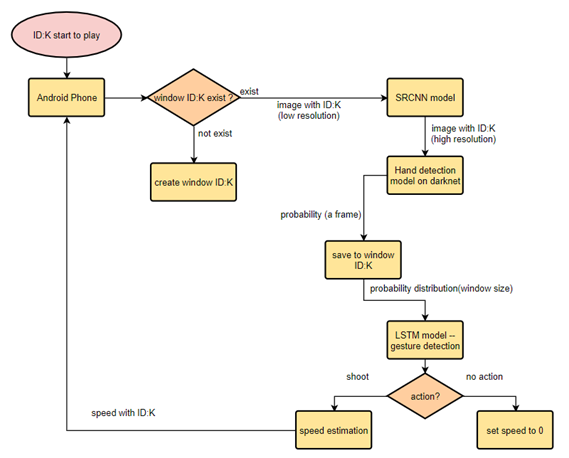
\includegraphics[width=10cm]{NN_SYS_structure.png}
    \caption{後端辨識系統架構圖}
    \label{fig:後端辨識系統架構圖}
\end{figure}

\subsubsection{SRCNN網路結構}
此處利用CNN神經網路將低解析度轉換為高解析度,以符合本地端訓練的照片高解析風格。以下呈現整體架構圖。

\begin{figure}[H]
    \centering
    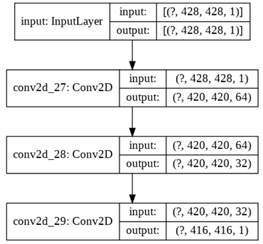
\includegraphics[width=6cm]{SRCNN_Structrue.png}
    \caption{SRCNN網路架構圖}
    \label{fig:SRCNN網路架構圖}
\end{figure}
\subsubsection{手部物件神經網路}

此專案是飛鏢遊戲,所以運算時間以及讀取時間需要降低,讓使用者不須等待就能得到射擊結果。
透過darknet平台,以yolov3為基礎更改其網路架構,以達成專屬類別輸出以及減少浮點運算次數的效果。並且,修改內部程式,達到傳輸效能提升,減少讀取時間。以下呈現經過多次實驗得到的新型網路架構。
\begin{figure}[H]
    \centering
    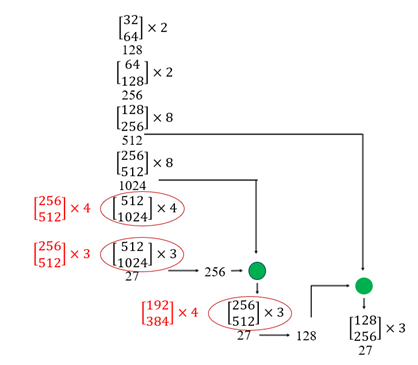
\includegraphics[width=8cm]{Darknet_Network.png}
    \caption{手部辨識神經網路架構圖(加速版)}
    \label{fig:手部辨識神經網路架構圖(加速版)}
\end{figure}



\subsubsection{LSTM神經網路}
手部物件辨識的機率分布存入window輸入至專門架設的LSTM網路結構中,並將輸出部份分為兩類別:無動作(0)、 射擊(1)。由於訓練資料的複雜度經過實驗後,發現並不需要使用更複雜的網路架構做學習,所以最終設計單層的LSTM。以下呈現LSTM網路架構。

\begin{figure}[H]
    \centering
    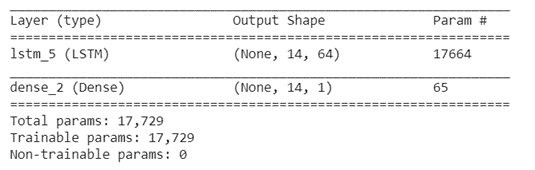
\includegraphics[width=8cm]{LSTM_Network.png}
    \caption{LSTM神經網路架構}
    \label{fig:LSTM神經網路架構}
\end{figure}


\subsection{神經網路實驗}

\subsubsection{優化darknet輸入評估實驗}

目的: 測試經過優化輸入後的darknet 與未優化輸入的darknet整體運作效能差距。
說明: 修改darknet中底層程式,並修改makefile後,重新編譯。讓darknet能加載numpy的內容,以及可以輸入陣列給darknet做偵測。而不需要再從硬碟讀取圖片作為輸入。
實驗方法:
\begin{itemize}
\item 實驗一未優化darknet輸入至原Yolo神經網路(未壓縮)做偵測。
\item 實驗二優化darknet輸入至原Yolo神經網路(未壓縮)做偵測。
\end{itemize}

測試方法:測試照片共100張的總時間,取平均時間。
\begin{figure}[H]
    \centering
    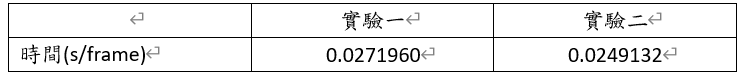
\includegraphics[width=10cm]{Darknet_Physics_Layer_OP.PNG}
    \caption{Darknet讀取優化比較}
    \label{fig:Darknet讀取優化比較}
\end{figure}
數據討論: 
每張降低0.00228秒,約 -8.4% 。	
結論: 
改採用優化darknet做為讀取輸入方式。


\subsubsection{神經網路手勢辨識實驗}

訓練資料生成:將訓練資料做resize成小圖片後再resize成原來大小。藉此產生訓練資料及測試資料。
訓練資料說明:兩張照片皆是由手機傳至伺服器後,重新resize成416*416大小(手部物件辨識網路輸入大小)。差別在於左側圖無經過SRCNN做高畫質轉換,而右側圖片有經過SRCNN做高畫質轉換。
將server照片經由SRCNN 轉換

\begin{figure}[H]
    \centering
    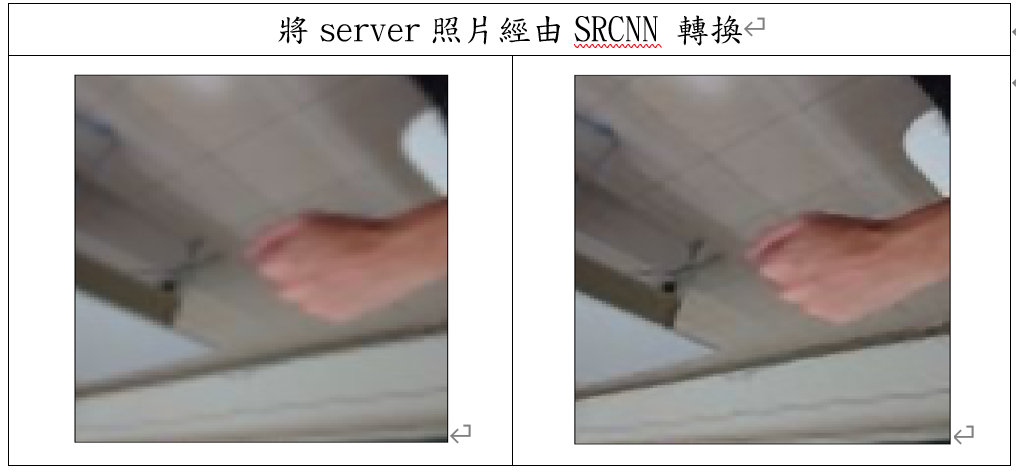
\includegraphics[width=10cm]{SRCNN_img.PNG}
    \caption{SRCNN效果圖呈現}
    \label{fig:SRCNN效果圖呈現}
\end{figure}

轉換結果評估:在未做SRCNN之前,手的輪廓並不明顯,影像顆粒度非常明顯。在做完SRCNN後,手的輪廓明顯從背景浮現,手上的陰影也更加明顯。

\subsubsection{未使用SRCNN測試結果}

\begin{figure}[H]
    \centering
    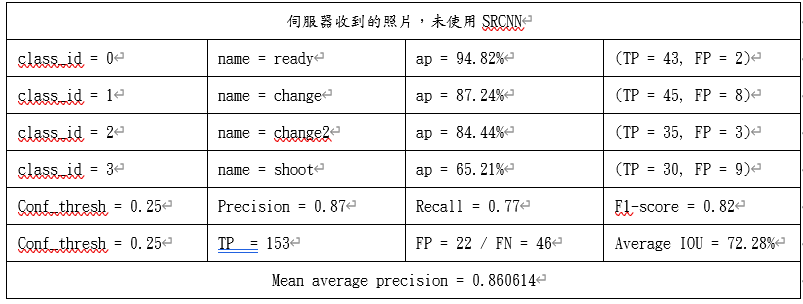
\includegraphics[width=10cm]{before_SRCNN_table.PNG}
    \caption{未使用SRCNN}
    \label{fig:未使用SRCNN}
\end{figure}

\subsubsection{使用SRCNN測試結果}

\begin{figure}[H]
    \centering
    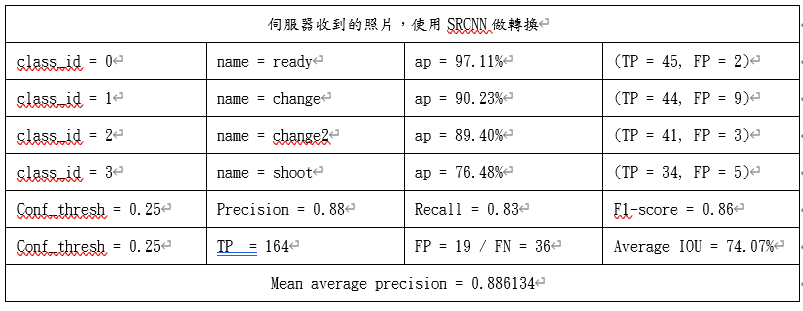
\includegraphics[width=10cm]{after_SRCNN_table.PNG}
    \caption{使用SRCNN}
    \label{fig:使用SRCNN}
\end{figure}

\begin{figure}[H]
    \centering
    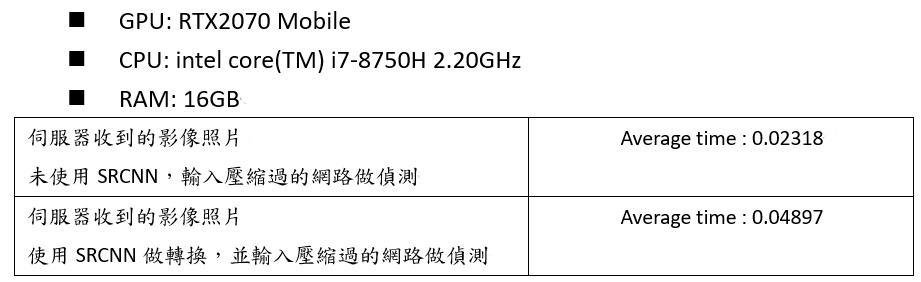
\includegraphics[width=10cm]{SRCNN_time.PNG}
    \caption{時間評估}
    \label{時間評估}
\end{figure}


評估:未做SRCNN之前,手的輪廓並不明顯,影像顆粒度非常明顯。做完SRCNN後,手的輪廓明顯從背景浮現,手上的陰影也更加明顯。使用SRCNN後mAP上升了2.5%。另外,做更深的細部分析。在最難判斷的類別id2、id3準確度皆有上升。推測可能是因為手的輪廓更明顯,從背景中凸顯出來,使手部物件辨識更加容易抓取手部位置,並更容易分類。另外,也沒有明顯的顆粒感在干擾CNN藉由filter擷取特徵的過程。
手部物件辨識:

\subsubsection{手部物件辨識網路訓練曲線圖}

\begin{figure}[H]
    \centering
    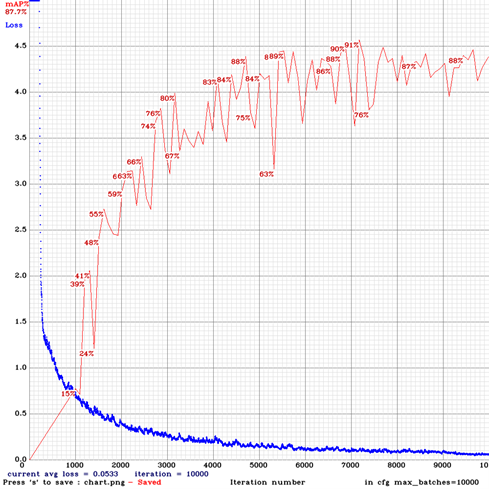
\includegraphics[width=10cm]{Darknet_Training_Curve_final.png}
    \caption{訓練曲線圖(Iteration)}
    \label{fig:訓練曲線圖(Iteration)}
\end{figure}

\begin{figure}[H]
    \centering
    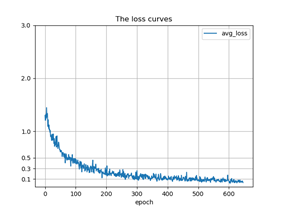
\includegraphics[width=10cm]{Darknet_Training_Curve2_final.png}
    \caption{訓練曲線圖(Epoch)}
    \label{fig:訓練曲線圖(Epoch)}
\end{figure}


觀察上方訓練結果,並沒有特別發現出現underfitting 或是 overfitting 的情形,雖然mAP以及loss在最後趨於穩定,表示其實learning rate 可以查是在做遞減,但是以整體訓練結果來看,validation data 測試所得的average mAP達到87.7%,表示訓練上收斂良好。

\subsubsection{新修改的CNN網路與原Yolo網路效能比較}

\begin{figure}[H]
    \centering
    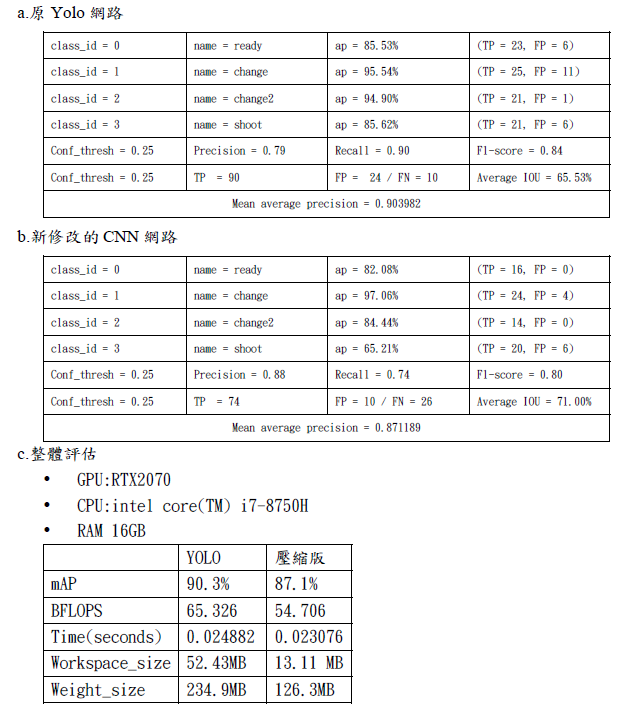
\includegraphics[width=15cm]{Darknet_Training_Table_final.PNG}
    \caption{}
    
\end{figure}




\subsubsection{window設計}

\begin{itemize}
\item X軸:單位時間
\item Y軸:次數
\end{itemize}

\begin{figure}[H]
    \centering
    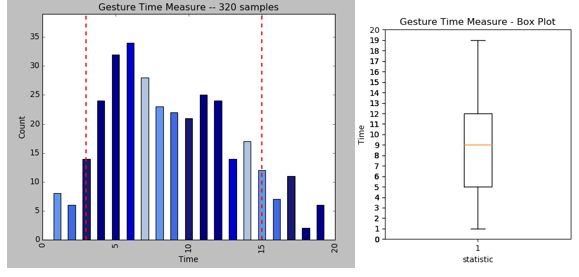
\includegraphics[width=10cm]{Windows_Size.PNG}
    \caption{}
\end{figure}

\subsubsection{LSTM網路設計實驗}

訓練資料生成:利用手部物件辨識得到的機率分布存成檔案,再將內部行數控制在window大小。由於資料不足,所以需要做資料擴充。利用random將機率做微調以及利用平移分布的方式,達到訓練資料擴充。
訓練資料共有500筆資料,切出200筆做為測試資料,評估模型。並將訓練資料由300筆增加至30000筆。

網路設計:
\begin{itemize}
\item 輸入維度  64 14 4
\item 將hidden state通過全連接層與sigmoid後輸出類別機率
\item 輸出機率0至1,threshold = 0.5,分為兩類發射(1)與無動作(0)
\item 學習率: Learning rate = 0.0001
\item 最佳化工具: Adam Optimizer
\item 損失函數: binary cross entropy
\item 未使用dropout
\item 訓練測試資料集比例0.8
\item 訓練次數100 epoch
\end{itemize}

\begin{figure}[H]
    \centering
    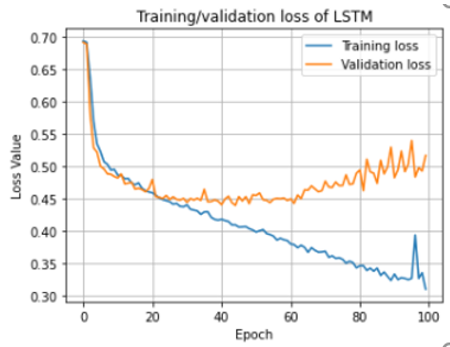
\includegraphics[width=10cm]{LSTM_Training_Curve.PNG}
    \caption{LSTM訓練曲線}
    \label{fig:LSTM訓練曲線}
\end{figure}

觀察上面Loss後,使用early stop技巧,將40 epoch 做為測試權重。
測試評估:使用真實資料100筆,各類別皆50筆,以避免資料分布不均導致評估不公正。

\begin{figure}[H]
    \centering
    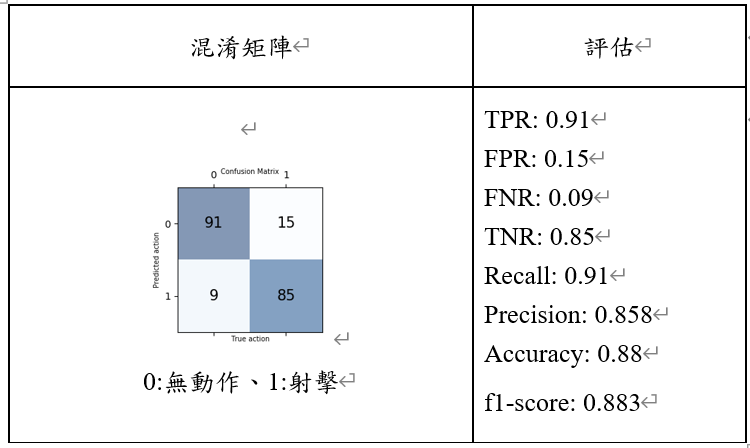
\includegraphics[width=10cm]{LSTM_Training_Table.PNG}
    \caption{手部辨識神經網路測試}
    \label{fig:手部辨識神經網路測試}
\end{figure}

分析:
由上面混淆矩陣,分類於第一類別(無動作)的正確率較高,而第二類別(射擊)的正確率相對較低。原因是,在製造第一類別(無動作)訓練資料時,可以將無動作訓練資料主要可以分為兩個類別,純粹無動作、或是有動作(但非射擊動作)。在第一部分純粹無動作是幾乎不會分類錯誤的,所以造成部份測試幾乎絕對正確。以至於第一類別(無動作)會正確率相較於第二類別(射擊)高。


\subsubsection{整體評估}
實驗方法:

使用200部影片,發射動作影片與無動作影片皆100部。給手部辨識神經網路辨識,辨識後根據該項實驗的設計來決定是否要傳送給SRCNN做高解析化,最後傳輸給LSTM網路做辨識。以LSTM網路辨識的準確度,以及整體辨識時間作為評估依據。

實驗設計:
\begin{itemize}
\item 實驗一:未優化darknet讀取影像照片方式
\item 未使用SRCNN + 未壓縮過後的手部辨識網路 + 單層LSTM輸出
\item 實驗二:優化darknet讀取影像照片方式
\item 未使用SRCNN + 未壓縮過後的手部辨識網路 + 單層LSTM輸出
\item 實驗三:優化darknet讀取影像照片方式
\item 未使用SRCNN + 壓縮過後的手部辨識網路 + 單層LSTM輸出
\item 實驗四:優化darknet讀取影像照片方式
\item 使用SRCNN + 壓縮過後的手部辨識網路 + 單層LSTM輸出
\end{itemize}

\begin{figure}[H]
    \centering
    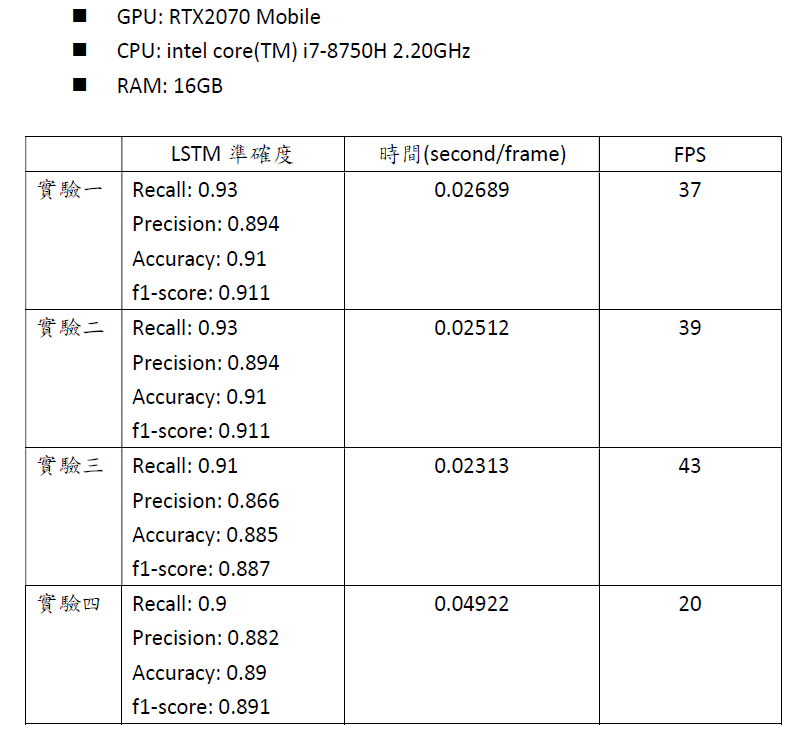
\includegraphics[width=10cm]{SUM_UP_EVAL.PNG}
    \caption{整體評估}
    \label{fig:整體評估}
\end{figure}


未壓縮優化的實驗一與加速優化的實驗三比較,FPS上升6。正確率卻只下降0.015。本專案在準確度達到一定要求下,會以縮短反應時間為主。因此選擇實驗三為本專題主要的偵測模式。
另外,對於額外使用SRCNN的實驗四來說,增加了高解析化後,雖然在(9)SRCNN實驗中顯示mAP上0.02,但是對於LSTM辨識結果並沒有太大作用,僅對於整體辨識結果正確率卻只上升0.05。而且辨識時間還增加一倍。因此往後的研究方向會以加速高解析化網路為主。

\begin{itemize}
\item 結論: 選擇實驗三作為目前專題的偵測模式。
\end{itemize}
